\documentclass[10pt]{book}
\usepackage[sectionbib]{natbib}
\usepackage{array,epsfig,fancyhdr,rotating}
\usepackage[driverfallback=dvipdfm]{hyperref}
\usepackage{soul} %for strikeout
%%%%%%%%%%%%%%%%%%%%%%%%%%%%%%%%%%%%%%%%%%%%%%%%%%%%%%%%%%%%%%%%%%%%%%%%%%%%%%%%%%%%%%%%%%%%%%%%%%%%%%%%%%%%%%%%%%%%%%%%%%%%

\textwidth=31.9pc
\textheight=46.5pc
\oddsidemargin=1pc
\evensidemargin=1pc
\headsep=15pt
%\headheight=.2cm
\topmargin=.6cm
\parindent=1.7pc
\parskip=0pt

\usepackage{amsmath}
\usepackage{amssymb}
\usepackage{amsfonts}
\usepackage{multirow}
\usepackage{amsthm}
\usepackage[export]{adjustbox}

\setcounter{page}{1}
\newtheorem{theorem}{Theorem}
\newtheorem{lemma}{Lemma}
\newtheorem{corollary}{Corollary}
\newtheorem{proposition}{Proposition}
\theoremstyle{definition}
\newtheorem{definition}{Definition}
%\newtheorem{proof}{Proof}
\newtheorem{example}{Example}
\newtheorem{remark}{Remark}
\pagestyle{fancy}

% List labels
\usepackage{scrextend}
\addtokomafont{labelinglabel}{\sffamily}

% Reference labels in the online appendix
\usepackage{xr}
\externaldocument{mdi-ss-supp}

%%%%%%%%%%%%%%%%%%%%%%%%%%%%%%%%%%%%%%%%%%%%%%%%%%%%%%%%%%%%%%%%%%%%%%%%%%%%%%%%%%%%%%%%%%%%%%%%%%%%%%%%%%%%%%%%%%%%%%%%%%%%
\pagestyle{fancy}
\def\n{\noindent}
\lhead[\fancyplain{} \leftmark]{}
\chead[]{}
\rhead[]{\fancyplain{}\rightmark}
\cfoot{}
\renewcommand{\headrulewidth}{0pt}

%%%%%%%%%%%%%%%%%%%%%%%%%%%%%%%%%%%%%%%%%%%%%%%%%%%%%%%%%%%%%%%%%%%%%%%%%%%%%%%%%%%%%%%%%%%%%%%%%%%%%%%%%%%%%%%%%%%%%%%%%%%%
%%%%%%%%%%%%%%%%%%%%%%%%%%%%%%%%%%%%%%%%%%%%%%%%%%%%%%%%%%%%%%%%%%%%%%%%%%%%%%%%%%%%%%%%%%%%%%%%%%%%%%%%%%%%%%%%%%%%%%%%%%%%

\begin{document}

%%%%%%%%%%%%%%%%%%%%%%%%%%%%%%%%%%%%%%%%%%%%%%%%%%%%%%%%%%%%%%%%%%%%%%%%%%%%%%%%%%%%%%%%%%%%%%%%%%%%%%%%%%%%%%%%%%%%%%%%%%%%
%%%%%%%%%%%%%%%%%%%%%%%%%%%%%%%%%%%%%%%%%%%%%%%%%%%%%%%%%%%%%%%%%%%%%%%%%%%%%%%%%%%%%%%%%%%%%%%%%%%%%%%%%%%%%%%%%%%%%%%%%%%%

\renewcommand{\baselinestretch}{2}

\markright{ \hbox{\footnotesize\rm Statistica Sinica
%{\footnotesize\bf 24} (201?), 000-000
}\hfill\\[-13pt]
\hbox{\footnotesize\rm
%\href{http://dx.doi.org/10.5705/ss.20??.???}{doi:http://dx.doi.org/10.5705/ss.20??.???}
}\hfill }

\markboth{\hfill{\footnotesize\rm JASON POULOS AND RAFAEL VALLE} \hfill}
{\hfill {\footnotesize\rm MISSING DATA IMPUTATION FOR SUPERVISED CLASSIFICATION} \hfill}

\renewcommand{\thefootnote}{}
$\ $\par

%%%%%%%%%%%%%%%%%%%%%%%%%%%%%%%%%%%%%%%%%%%%%%%%%%%%%%%%%%%%%%%%%%%%%%%%%%%%%%%%%%%%%%%%%%%%%%%%%%%%%%%%%%%%%%%%%%%%%%%%%%%%

\fontsize{12}{14pt plus.8pt minus .6pt}\selectfont \vspace{0.8pc}
\centerline{\large\bf MISSING DATA IMPUTATION }
\vspace{2pt} \centerline{\large\bf  FOR SUPERVISED CLASSIFICATION}
\vspace{.4cm} \centerline{Jason Poulos and Rafael Valle} \vspace{.4cm} \centerline{\it
University of California, Berkeley} \vspace{.55cm} \fontsize{9}{11.5pt plus.8pt minus
.6pt}\selectfont

%%%%%%%%%%%%%%%%%%%%%%%%%%%%%%%%%%%%%%%%%%%%%%%%%%%%%%%%%%%%%%%%%%%%%%%%%%%%%%%%%%%%%%%%%%%%%%%%%%%%%%%%%%%%%%%%%%%%%%%%%%%%

\begin{quotation}
\noindent {\it Abstract:}
This paper compares methods for imputing missing categorical data for classification
tasks using random forests, decision trees and deep neural networks.
Researchers analyzing survey data typically choose decision trees or random
forests for classification tasks, largely because these models, unlike neural
networks and others, do not require imputing missing data nor encoding categorical
variables. We start by investigating techniques for missing categorical data imputation
and categorical data encoding. We experiment on two benchmark datasets with missing categorical data, comparing the three classifiers trained on either non-imputed or differently imputed data with different degrees of nonmissing at random (MNAR) perturbation. We beat the state-of-the-art test error on both datasets and conclude from the results that the performance of the classifiers and imputation strategies generally depend on the nature and proportion of missing data. \par

\vspace{9pt}
\noindent {\it Key words and phrases:}
missing data, survey data, imputation methods,  neural networks,  deep learning, random forests, decision trees, prediction intervals
\par
\end{quotation}\par



\def\thefigure{\arabic{figure}}
\def\thetable{\arabic{table}}

\fontsize{12}{14pt plus.8pt minus .6pt}\selectfont

\newpage %move intro to second page

\setcounter{chapter}{1}
\setcounter{equation}{0} %-1
\noindent {\bf 1. Introduction} 

Missing data is a common problem in survey data in various domains, such as social science and marketing. Sources of missing data in surveys include nonresponse and attrition in longitudinal surveys. For supervised classification tasks, the objective is to fit a model on categorically labeled training data in order to categorize new examples. The ability of researchers to accurately fit a model model may be compromised by missing data, depending on the underlying missing data mechanism. In this paper, we focus on data that are missing not at random (MNAR), which occurs when the probability of an example having a missing value may depend on the missing data itself. There is an inherent nonidentifiability problem when the missing data mechanism is MNAR because we cannot observe the true value of missing data \citep{tsiatis2007}. Item nonresponse in surveys is typically handled by imputation methods, which are used to estimate a value for missing data. However, imputation methods assume data missing at random (MAR), which occurs when the probability of missingness depends only on the observed data. 

The objective of the present study is to compare the out-of-sample performance of three popular machine learning classifiers --- decision trees, random forests, and neural networks --- trained on either differently-imputed or non-imputed survey datasets that contain various degrees of MNAR missing data. Decision trees and random forests are typically used for survey data because missing data must be pre-processed to be suited for models that require numerical input, such as neural networks. Imputation methods that assume data at MAR when the data is in fact MNAR can bias model estimates. The results of the study will provide guidance to applied researchers on how to handle missing data in survey datasets and which classifier to use. 

This manuscript is organized as follows: Section 2 describes missing data mechanisms and describe methods imputing missing data; Section 3 describes our experiments on two benchmark datasets and discusses the results; Section 4 concludes and offers areas for future research. 

\par

\lhead[\footnotesize\thepage\fancyplain{}\leftmark]{}\rhead[]{\fancyplain{}\rightmark\footnotesize\thepage}%Put this line in Page 2

\setcounter{chapter}{2}
\setcounter{equation}{0} %-1
\noindent {\bf 2. Missing data and imputation methods}

In this section, we describe the missing data mechanisms underlying patterns of missing data common to survey datasets. We then review popular methods of handling missing data.

\par
\noindent {\bf 2.1. Missing data patterns and mechanisms}

It is important to first distinguish between missing data patterns, which describe which values are observed and which are missing, and missing data mechanisms, which describe the the probability of missingness  \citep{little2014}. Common missing data patterns in surveys typically include unit nonresponse, where a subset of participants do not complete the survey, and item nonresponse, where missing values are concentrated on particular questions. In opinion polls, nonresponse may reflect either refusal to reveal a preference or lack of a preference \citep{de2003prevention}. 

It may be beneficial to impute missing values in situations where missing data hide values that are useful for classification tasks. Understanding the missing data mechanisms underlying patterns of missing data is crucial since properties of imputation methods depend on the nature of these mechanisms. Following the notation of \cite{little2014}, let $Y = y_{ij}$ be a $(n \times K)$ dataset with each example $y_i = (y_{i1}, \ldots, y_{iK})$ the set of $y_{ij}$ values of feature $Y_j$ for example $i$. Let $Y_{\mathrm{obs}}$ define observed values of $Y$ and $Y_{\mathrm{mis}}$ define missing values. Define the missing data identity matrix $M = m_{ij}$, where $m_{ij} = 1$ if $y_{ij}$ is missing and $m_{ij} = 0$ if $y_{ij}$ is nonmissing. The missing data mechanism is called missing completely at random (MCAR) if the probability of missingness is independent of the data, or $f(M | Y, \phi) = f(M | \phi)$, where $\phi$ denotes unknown parameters. The MAR assumption is less restrictive than MCAR in that that the probability of missingness depends only on the observed data, $f(M | Y, \phi) = f(M | Y_{\mathrm{obs}}, \phi)$. We are primarily interested in the MNAR assumption that the probability of missingness may also depend on the unobserved data, 

\begin{equation}\label{2.1}
f(M | Y, \phi) = f(M | Y_{\mathrm{mis}}, \phi) \hspace{5mm} \forall \,Y_{\mathrm{mis}}, \phi.
\end{equation} Researchers typically assume data is MAR, which mitigates the identifiability problems of MNAR because the probability of missingness depends on the features that are observed on all individuals \citep{tsiatis2007}. 

\par			
\noindent {\bf 2.2. Imputation methods} \label{section:techniques} 

Complete-case analysis (i.e., simply discarding examples with missing values) is wasteful of information and will bias estimates unless the data are MCAR. Since there is no way to distinguish whether the missing data are MCAR or MNAR from the observed data, a natural strategy is to impute missing values and then proceed as if the imputed values are true values. Imputation methods that rely on explicit model assumptions include \emph{mean or mode replacement}, which substitutes missing values with the mean (for quantitative features) or mode (for qualitative features) of the feature vector, and \emph{prediction model} imputation, which replaces missing values with the predicted values from a regression of $Y_{\mathrm{mis}}$ on $Y_{\mathrm{obs}}$. Explicit modeling methods assume the data are MAR while implicit modeling methods, which are algorithmic in nature and rely only on implicit assumptions, generally do not assume the underlying missing data mechanism. Implicit methods include \emph{random replacement}, where an example with missing data is randomly replaced with another complete example randomly sampled, and \emph{hot deck} imputation, where missing values are replaced by ``similar'' nonmissing values. Hot deck imputation can be implemented by computing the $k$-nearest-neighbors ($k$-NN) of an example with missing data and assigning the mode of the $k$-neighbors to the missing data. \citep{batista2003analysis} use this procedure and find $k$-NN imputation can outperform internal methods used by decision trees to treat missing data and summary statistic imputation. \citep{li2004} propose a hot deck imputation method based on fuzzy $k$-means. 

\citep{silva2011} empirically compare imputation based on using artificial neural networks (ANNs) with mean/mode  imputation, regression models (logistic regression and multiple linear regression), and hot deck, and find the ANNs model performs the best on datasets with categorical variables. 

\par
\noindent {\bf 2.3. One-hot encoding for missing data} 

A natural strategy in dealing with missing data for supervised learning problems is one-hot encoding. Instead of imputing missing data, one-hot encoding creates a binary feature vector that indicates missing values. For categorical features, one-hot encoding simply treats a missing value symbol (e.g, ``?") as a category when the categorical features are binarized. For continuous features, missing values are set to a constant value and a missingness indicator is added to the feature space. One-hot encoding for missing data yields biased estimates when the features are correlated, which is often the case with survey data, even when data are MCAR \citep{jones1996}. 

\par

%%%%%%%%%%%%%%%%%%%%%%%%%%%%%%%%%%%%%%%%%%%%%%%%%%%%%%%%%%%%%%%%%%%%%%%%%%%%%%%%%%%%%%%%%%%%%%%%%%%%%%%%%%%%%%%%%%%%%%%%%%%%
%\newpage

\setcounter{chapter}{3}
\setcounter{equation}{0} %-1
\noindent {\bf 3. Experiments} 

In this section, we describe our experiment on two benchmark datasets with missing categorical data, comparing three popular classifiers (neural networks, decision trees, and random forests) trained on either non-imputed or differently imputed data with different degrees of MNAR perturbation.

\par
\noindent {\bf 3.1. Benchmark datasets}

We experiment on two benchmark datasets from the UCI Machine Learning Repository: the Adult dataset and Congressional Voting Records (CVRs) dataset \citep{Lichman2013}. The Adult dataset contains $N=48,842$ examples and 14 features (6 continuous and 8 categorical). Missing values in this dataset are survey nonresponses. The prediction task is to determine whether a person makes over \$50,000 a year. The CVRs dataset contains $N=435$ examples, each the voting record of a member of the $98^{th}$ U.S. House of Representatives for 16 key roll call votes. The dataset contains 16 categorical features with three possible values: ``yea'', ``nay'', and missing. Missing values in this dataset are not simply unknown, but represent values other up-or-down votes, such as voted present, voted present to avoid conflict of interest, and did not vote or otherwise make a position known. The prediction task is to classify party affiliation (Republican or Democrat). 

We randomly split each dataset $2/3$ for training and $1/3$ for testing. The state--of--the--art for the Adult dataset is a Naive Bayes classifier that achieves a 14.05\% generalization error after removing examples with missing values \citep{kohavi1996}. The CVRs dataset donor claims to achieve a 90-95\% accuracy using an incremental decision tree algorithm called STAGGER, although it is not known what train-test split is used or how missing values are handled \citep{schlimmer1987,schlimmer1986}.

\par
\noindent {\bf 3.2. Patterns of missing data}

Uncovering missing data patterns in the datasets is will help to identify possible missing data mechanisms and select appropriate imputation methods. In the supplementary material (SM), Figure SM-\ref{fig:proportion-missing-adult} analyzes patterns of missing data in the Adult dataset, in which 7\% of the examples contain missing values. Missing data in the Adult dataset is due to item nonresponse, as missing values are concentrated in three of the categorical features --- \emph{Work class}, \emph{Occupation}, and \emph{Native country}--- and no examples contain entirely missing data. It is unlikely that the data are MCAR because observations that are missing in \emph{Work class} are also missing in \emph{Occupation} (about 6\% of examples have missing values in both). About 1\% of examples are missing just \emph{Native country} and less than 1\% are missing all three features. There is no way to determine from the observed data whether the missing data are MAR or MNAR; the data are MNAR if the probability of missingness cannot be explained only by the observed data in the other predictors.

Close to half of the CVRs data contains missing values, which are present in every feature (Figure SM-\ref{fig:proportion-missing-votes}). About a quarter of missing data is in \texttt{South Africa}, which was a controversial amendment to amend the Export Administration Act to bar U.S. exports to South Africa's apartheid regime. Twelve percent of missing data is in the feature \texttt{Water}, which is a water projects authorizations bill, and 7\% of missing data rests in the feature \texttt{Exports}, which is a tariff bill. The data are unlikely to be MCAR because 12\% of the data are missing in just \texttt{South Africa} and less than 1\% of examples are missing across all features. It is most likely in this case that the CVRs data are MNAR because the probability of missing a vote or voting present on one important bill should not theoretically be influenced by observed votes on other important bills. 

\par
\noindent {\bf 3.3. Preprocessing}

In order to study the effect of larger amounts of missing data, we perturb the training data so that each categorical feature has 10\%, 20\%, 30\%, and 40\% values missing according to the MNAR mechanism
 
 \begin{equation}\label{3.1}
\Pr (M_i = 1 | y_i, \phi) = \begin{cases}
1, &\text{if $y_i \in A$ \hspace{5mm} $\forall \,$ categorical $Y_j$} \\
0, &\text{if $y_i \notin A$ \hspace{5mm} $\forall \,$ categorical $Y_j$},
\end{cases}
\end{equation} where $A$ is a vector containing at least one value from each categorical feature that we determine likely to be missing. We select categorical values in the Adult dataset that are theoretically correlated with low socioeconomic status, such as the values ``Without pay'' and ``Never worked" for the feature \emph{Work class}. The existing literature suggests item nonresponse in surveys is correlated with low income and low education \citep{rubin1995}. We include in $A$ only ``nay'' votes, under the assumption that refusing to take position on an issue or missing a vote is akin to voting against the issue. 

After one-hot encoding the categorical variables in the training data, we implement each of the following imputation techniques, discussed in Section 2.2: $k$-NN, prediction model (logistic regression, random forests, or SVMs), mode replacement, and random replacement. We then standardize continuous features by subtracting the mean and dividing by the standard deviation of the feature. The test data is preprocessed in the same manner, with the exception that we do not perturb categorical features in the test data.%\footnote{When imputing the missing data with mode replacement, we use the training set mode. We also use the training set mean and standard deviation to standardize test set features.}

\par
\noindent {\bf 3.4. Model training and assessment}

We train three different classifiers on the preprocessed data: decision trees, random forests, and deep neural networks. The deep neural network consists of four layers, each of the two hidden layers having 1024 nodes, and employs the adaptive learning rate method Adadelta \citep{zeiler2012} for the update rule. We explore the following hyperparameter space via Bayesian optimization \citep{snoek2012}: Momentum schedule (0 to 1), dropout regularization (No, Yes) and learning rate: (0.000001 to 0.01). We obtain an ensemble of different candidate models that minimize training error during Bayesian optimization. 

We construct prediction confidence intervals using the variation in an ensemble of neural networks, each model fit on the training data and applied to the test data \citep{heskes1997}. We use the same procedure for decision trees and random forests, creating an ensemble of decision trees by varying the maximum depth of the tree (5 to no maximum, i.e., nodes are expanded until all leaves are pure), and an ensemble of random forests by varying the number of trees for random forests (10 to 2,000) and the number of features to consider when looking for the best split (the square root, logarithm, or total number of features). 

\par
\noindent {\bf 3.5. Results}

We assess the performance of the neural network classifier in terms of test set error rate in comparison with decision tree and random forests classifiers on differently imputed data and for various degrees of perturbation.  We use one-hot encoding to represent missing data when no imputation method is used. The results on the Adult dataset and CVRs dataset are plotted in Figures \ref{fig:test-error-adult} and \ref{fig:test-error-votes}, respectively. For the Adult dataset, the random forests classifier trained on data imputed with logistic regression yields the lowest generalization error (13.85\% error), beating the state-of-the-art by 0.2\%. In comparison, random forests trained on data with no missing data imputation matches the state-of-the-art (14.05\%) and neural network trained on data imputed by random replacement performs considerably worse (14.37\%). For the CVRs dataset, random forests trained on one-hot encoded data with up to 20\% of the data perturbed beats the state-of-the-art by over 2\% (2.77\%). Neural networks trained on PCA-imputed data or no imputation also beat the state-of-the-art, with error rates of 3.47\% and 4.16\%, respectively. 

Overall, the performance of the classifiers and imputation strategies depend on the dataset and amount of missing data. For the Adult dataset, random forests classifiers trained on data imputed with other classifiers (i.e., logistic regression, random forests, and SVMs) outperform other classifiers and imputation methods across different ratios of perturbed data. All classifiers trained on one-hot encoded data perform very poorly when the Adult dataset is perturbed. This is likely due to the fact that in the original, non-perturbed Adult dataset, missing values are concentrated in three features which may not be consequential for the prediction task. Perturbation exposes features that are more consequential to the prediction task to missing data. 

Each of the three classifiers trained on one-hot encoded data perform well on the CVRs dataset. In this dataset, missing values represent potentially valuable information for the prediction task and can be more useful for the classifier than the imputed value for certain features. This is why it is not implausible that a classifier trained on perturbed, one-hot encoded data can have lower generalization error than a classifier trained on non-perturbed, one-hot encoded data. 

\begin{figure}[h!]
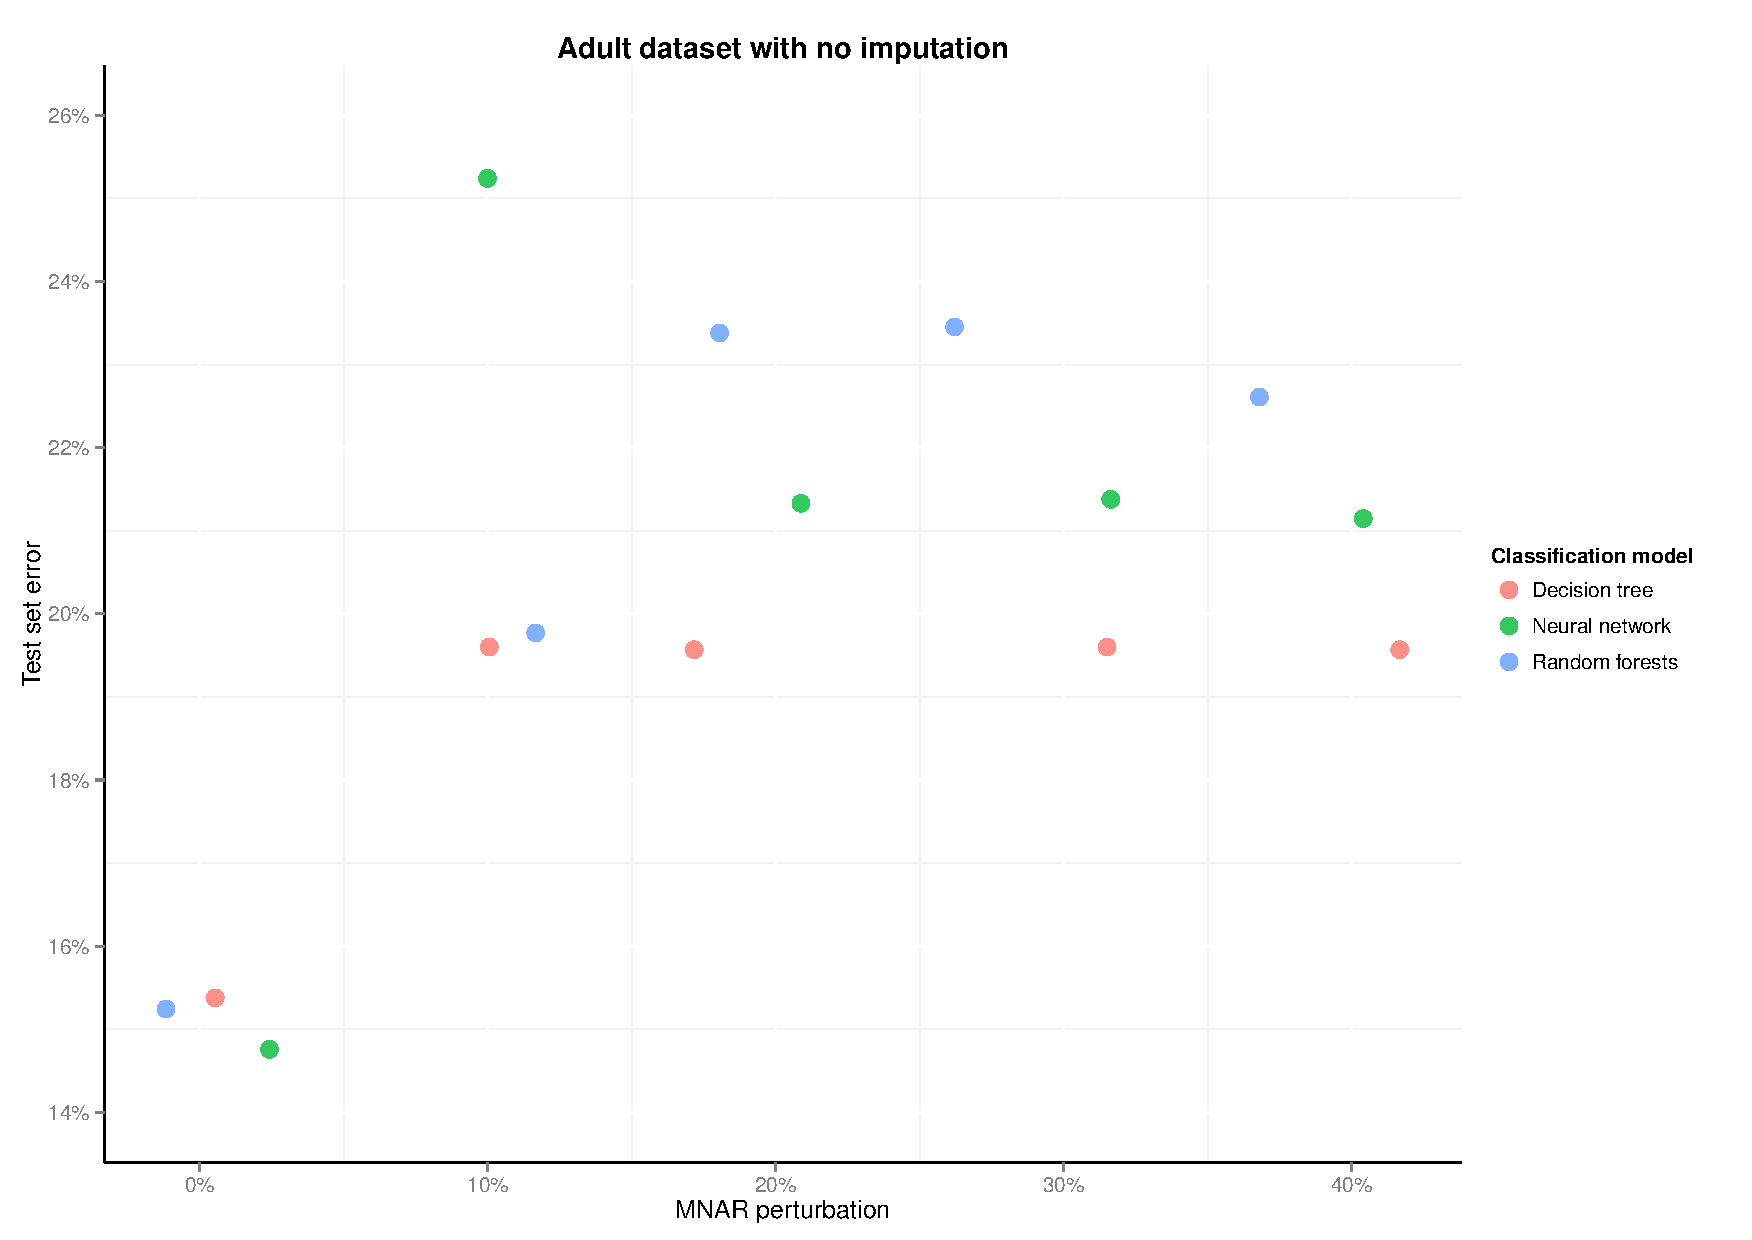
\includegraphics [scale=0.45]{figure/test-errors-adult-no-imp.pdf}\par
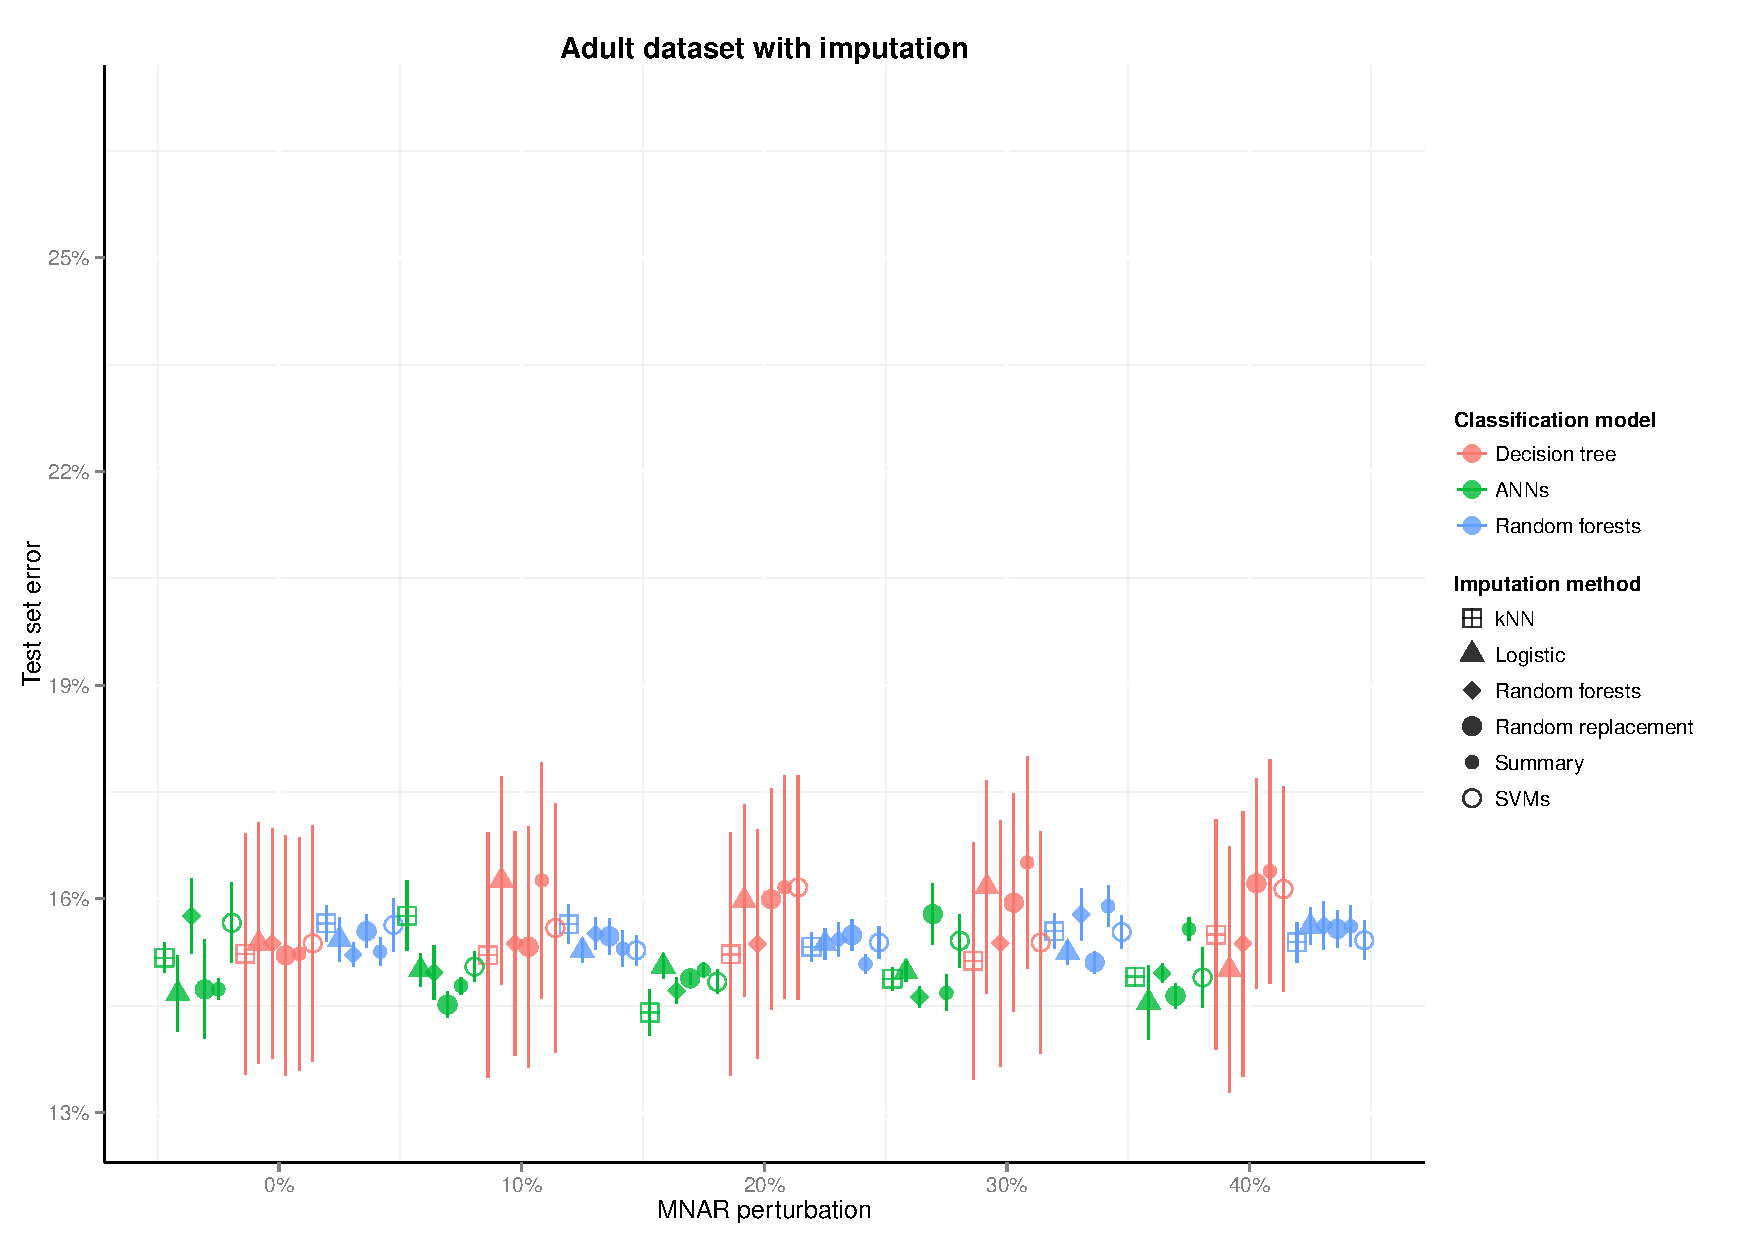
\includegraphics [scale=0.45]{figure/test-errors-adult-imp.pdf}\par
   \caption{\footnotesize Error rates on the Adult test set with (bottom) and without (top) missing data imputation, for various levels of perturbed training features (x-axis). One-hot encoding is used to represent missing data in the absence of imputation.}
   \label{fig:test-error-adult}
\end{figure}

\begin{figure}[h!]
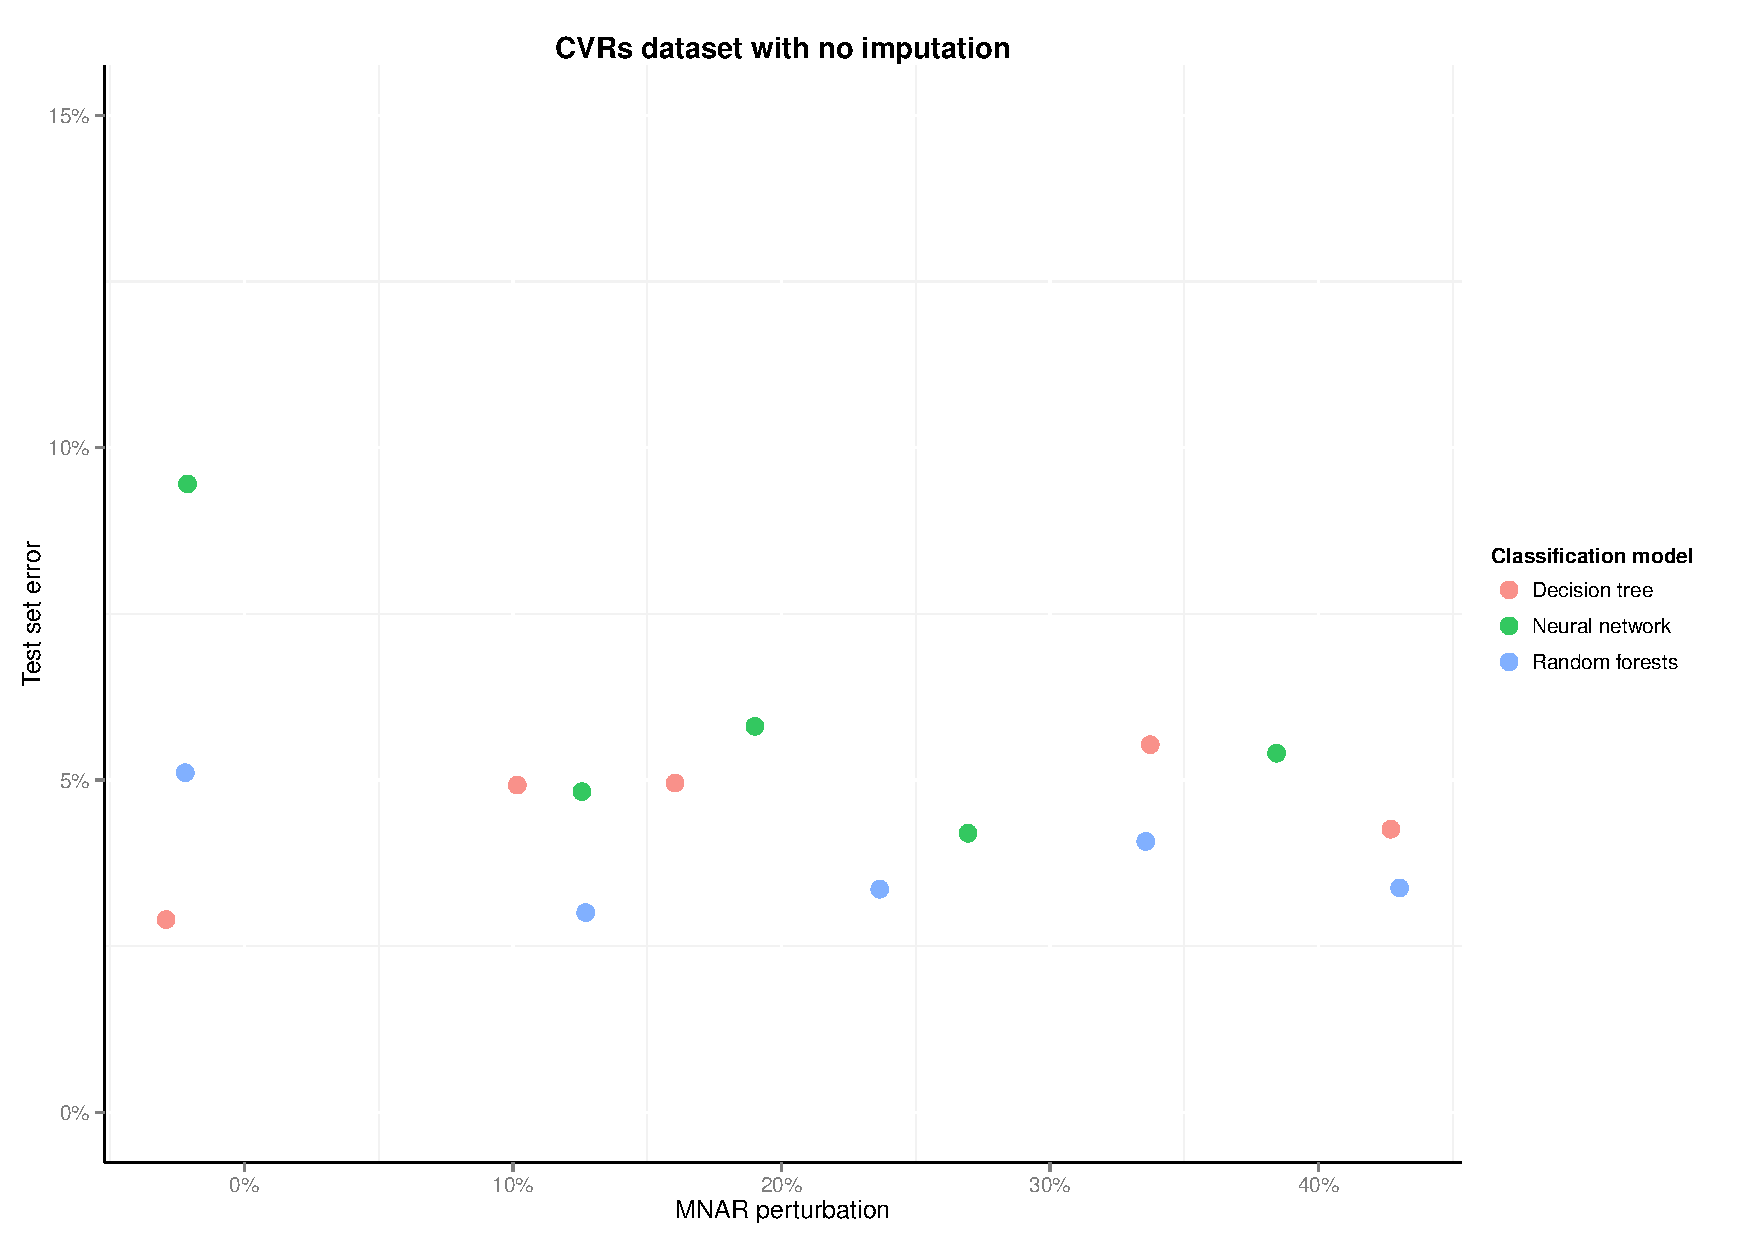
\includegraphics [scale=0.45]{figure/test-errors-votes-no-imp.pdf}\par
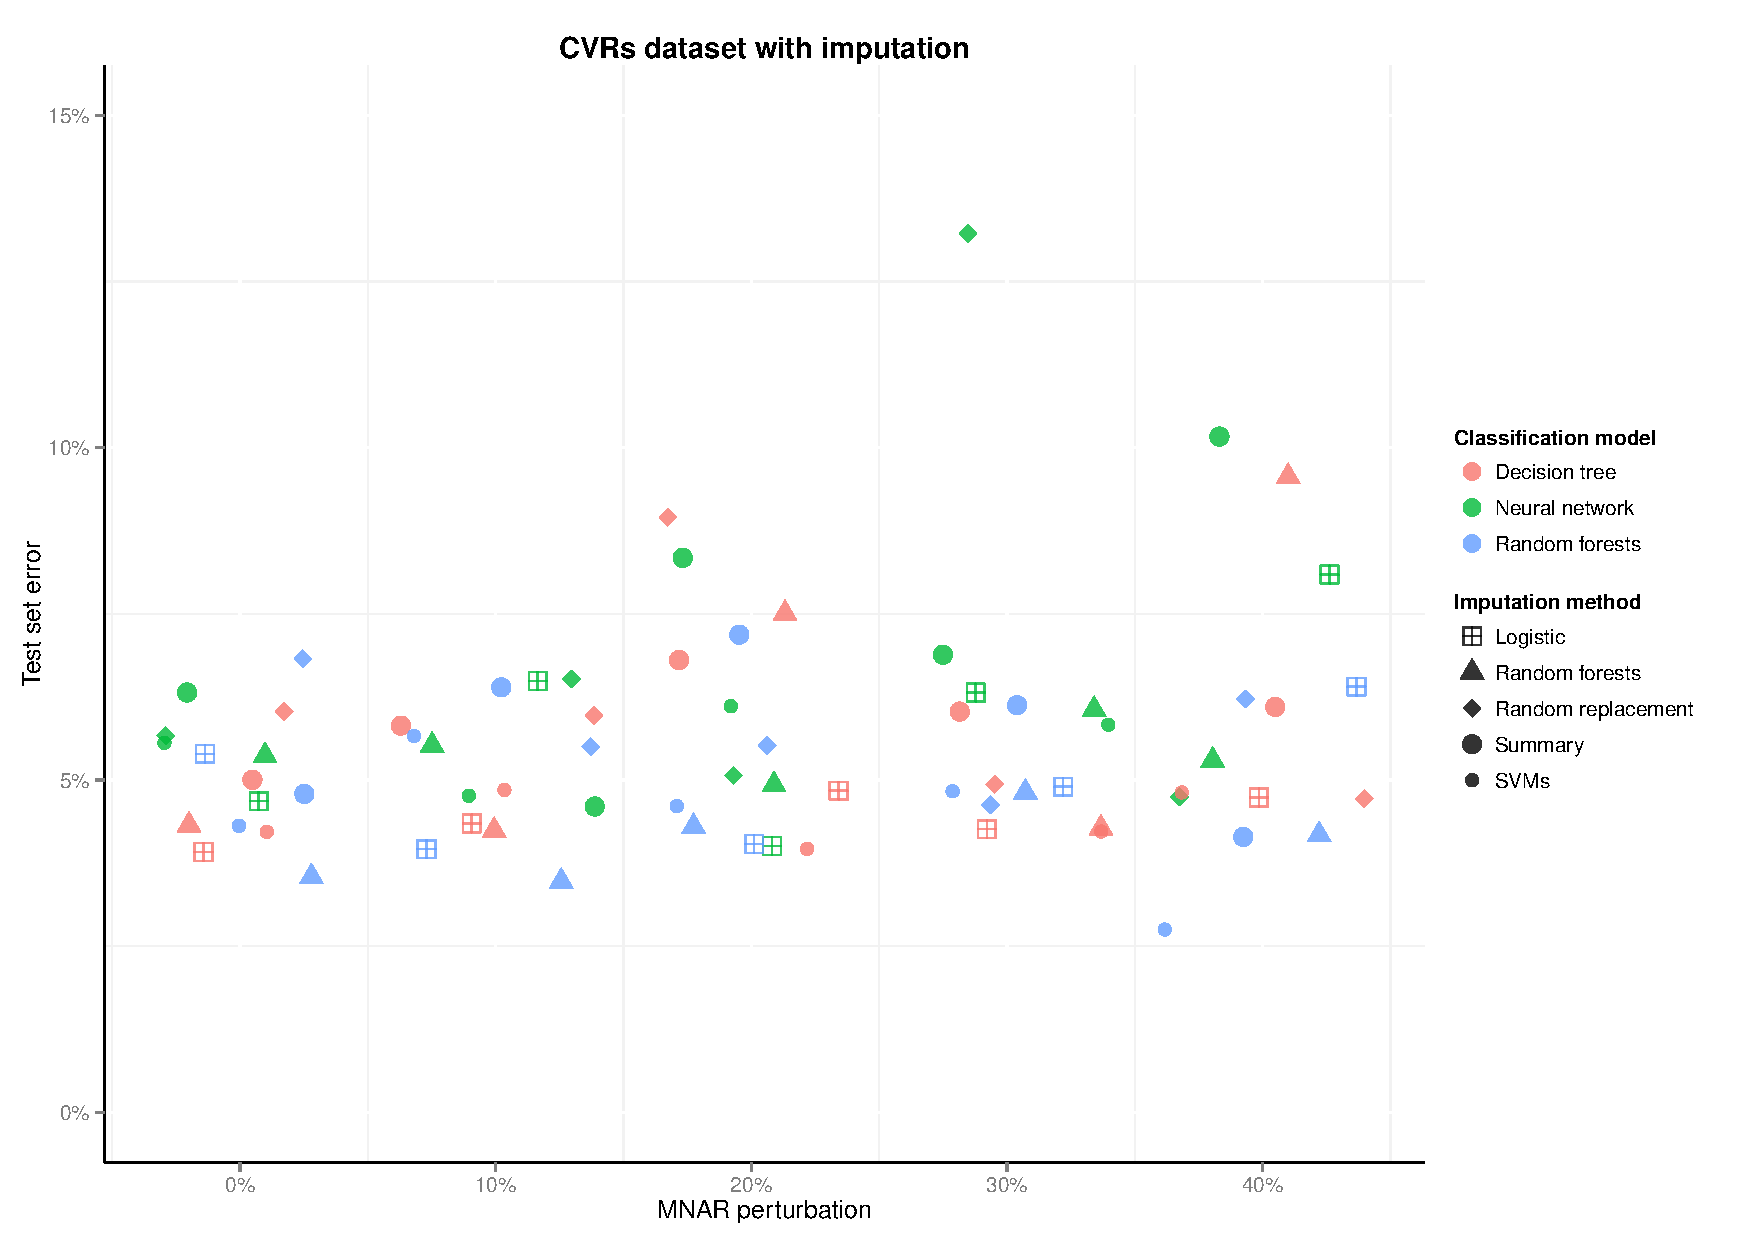
\includegraphics [scale=0.45]{figure/test-errors-votes-imp.pdf}\par
   \caption{\footnotesize Error rates on the CVRs test set with (bottom) and without (top) missing data imputation. See footnotes for Figure \ref{fig:test-error-adult}.}
   \label{fig:test-error-votes}
\end{figure}

\par

\setcounter{chapter}{4}
\setcounter{equation}{0} %-1
\noindent {\bf 4. Conclusion}  

Neural networks have become a popular machine learning algorithm in many domains, in part due to the ability of neural networks to ``learn'' how to engineer features.  However, researchers analyzing survey data typically choose decision trees or random forests for prediction tasks because missing data and categorical variables are not easy to handle with neural networks. This paper investigates techniques for handling missing data for training neural network classifiers. 

We compare the predictive performance of a four-layer neural network against decision tree and random forest classifiers trained on datasets with differently imputed data. We assess performance in terms of test set error for different levels of perturbed training data, from 0\% (no perturbation) to 40\% perturbation. We beat the state-of-the-art test error on the Adult dataset by 0.2\% using a random forests classifier trained on data imputed with logistic regression. Random forests trained on perturbed and one-hot encoded data outperforms the state-of-the-art on the CVRs dataset by over 2\%. 

We conclude from the results that the performance of the classifiers and imputation strategies generally depend on the nature and proportion of missing data. For the Adult dataset, random forests classifiers trained on data imputed with other classifiers outperform other classifiers and imputation methods across different ratios of perturbed data, while classifiers trained on one-hot encoded data perform very poorly on perturbed training data. This finding can be explained by the fact that missing values in the Adult dataset are concentrated in three features which may not be consequential for the prediction task, and perturbation exposes features that are more consequential to the prediction task to missing data. For the CVRs dataset, each of the three classifiers trained on one-hot encoded data perform well across different levels of perturbation. This finding can be explained by the fact that missing values represent potentially valuable information for the prediction task in the CVRs data.

For future work, we will further explore the idea that missing data may have more predictive value than imputed data in certain domains. A related question is whether neural networks can outperform decision trees or random forests trained on one-hot encoded data by learning different types of missing values. For instance, can neural networks engineer features that reflect the different types of missing values in the CVRs data, where missing values represent any action other than an up-or-down vote (e.g., voted present)? Answers to these questions will help guide researchers in choosing which imputation strategies and classifiers to use for prediction problems in different domains. 
\par
%%%%%%%%%%%%%%%%%%%%%%%%%%%%%%%%%%%%%%%%%%%%%%%%%%%%%%%%%%%%%%%%%%%%%%%%%%%%%%%%%%%%%%%%%%%%%%%%%%%%%%%%%%%%%%%%%%%%%%%%%%%%
\vskip 14pt
\noindent {\large\bf Supplementary Materials}

%Contain the brief description of the online supplementary materials.
The online supplementary material contains descriptive plots of missing data patterns in the benchmark datasets, as well as a description and plots of Bayesian hyperparameter optimization for training neural networks on the benchmark datasets. The code used for this project is available on Github (\url{https://github.com/rafaelvalle/MDI}).

\par
%%%%%%%%%%%%%%%%%%%%%%%%%%%%%%%%%%%%%%%%%%%%%%%%%%%%%%%%%%%%%%%%%%%%%%%%%%%%%%%%%%%%%%%%%%%%%%%%%%%%%%%%%%%%%%%%%%%%%%%%%%%%
\vskip 14pt
\noindent {\large\bf Acknowledgements}

%Write the acknowledgements here.
We thank Isabelle Guyon for advice and the idea for the paper. We also thank Joan Bruna and seminar participants at the University of California, Berkeley, for comments. This material is based upon work supported by the National Science Foundation Graduate Research Fellowship under Grant No. DGE 1106400. Any opinion, findings, and conclusions or recommendations expressed in this material are those of the authors and do not necessarily reflect the views of the National Science Foundation.
\par

%%%%%%%%%%%%%%%%%%%%%%%%%%%%%%%%%%%%%%%%%%%%%%%%%%%%%%%%%%%%%%%%%%%%%%%%%%%%%%%%%%%%%%%%%%%%%%%%%%%%%%%%%%%%%%%%%%%%%%%%%%%%
\markboth{\hfill{\footnotesize\rm JASON POULOS AND RAFAEL VALLE} \hfill}
{\hfill {\footnotesize\rm MISSING DATA IMPUTATION FOR SUPERVISED CLASSIFICATION} \hfill}

\bibhang=1.7pc
\bibsep=2pt
\fontsize{9}{14pt plus.8pt minus .6pt}\selectfont
\renewcommand\bibname{\large \bf References} 
\clearpage
\markboth{\hfill{\footnotesize\rm JASON POULOS AND RAFAEL VALLE} \hfill}
{\hfill {\footnotesize\rm MISSING DATA IMPUTATION FOR SUPERVISED CLASSIFICATION} \hfill}
%\begin{thebibliography}{11}
%\expandafter\ifx\csname
%natexlab\endcsname\relax\def\natexlab#1{#1}\fi
%\expandafter\ifx\csname url\endcsname\relax
%  \def\url#1{\texttt{#1}}\fi
%\expandafter\ifx\csname urlprefix\endcsname\relax\def\urlprefix{URL
%}\fi
%\bibitem[Antoine and Renault(2012)]{1} Antoine, B. and Renault, E. (2012). Efficient minimum distance
%estimation with multiple rates of convergence. \textit{J. Economet.} \textbf{170}, 350-367.
%\bibitem[Shao and Tu(1995)]{2}
%Shao, J. and Tu, D. (1995). \textit{The Jackknife and Bootstrap}. Springer-Verlag, New York.
%
%%%%%%%%%%%%%%%%%%%%%%%%%%%%%%%%%%%%%%%%%%%%%%%%%%%%%%%%%%%%%%%%%%%%%%%%%%%%%%%%%%%%%%%%%%%%%%%%%%%%%%%%%%%%%%%%%%%%%%%%%%%%%
%\end{thebibliography}
\bibliographystyle{apalike}
\bibliography{refs}

\vskip .65cm
\noindent
Department of Political Science, University of California, Berkeley, CA 94720-1950
\vskip 2pt
\noindent
E-mail: \href{mailto:poulos@berkeley.edu}{\nolinkurl{poulos@berkeley.edu}}
\vskip 2pt

\noindent
Center for New Music and Audio Technologies, University of California, Berkeley, CA 94720
\vskip 2pt
\noindent
E-mail: \href{mailto:rafaelvalle@berkeley.com}{\nolinkurl{rafaelvalle@berkeley.com}}
% \vskip .3cm
%\centerline{(Received ???? 20??; accepted ???? 20??)}\par
\end{document}
%%%%%%%%%%%%%%%%%%%%%%%%%%%%%%%%%%%%%%%%%%%%%%%%%%%%%%%%%%%%%%%%%%%%%%%%%%%%%%%%%%%%%%%%%%%%%%%%%%%%%%%%%%%%%%%%%%%%%%%%%%%%
%%%%%%%%%%%%%%%%%%%%%%%%%%%%%%%%%%%%%%%%%%%%%%%%%%%%%%%%%%%%%%%%%%%%%%%%%%%%%%%%%%%%%%%%%%%%%%%%%%%%%%%%%%%%%%%%%%%%%%%%%%%%

\end{document}
